\chapter{The Cauchy--Kovalevskaya theorem}\label{chapter:Cauchy.Kovalevskaya}%
\chapterSummary{We prove the Cauchy--Kovalevskaya theorem: analytic determined systems of partial differential equations have local solutions, with arbitrary initial conditions.}%
\section{Formal Taylor series}
For \(x_1,x_2,\dots,x_n\) real variables and \(a_1,a_2,\dots,a_n\) nonnegative integers, let
\begin{align*}
x&\defeq(x_1,x_2,\dots,x_n),\\
a&\defeq(a_1,a_2,\dots,a_n),\\ 
x^a&\defeq x_1^{a_1} \dots x_n^{a_n},\\
a!&\defeq a_1!\dots a_n!\text{ and}\\ 
\partial^a&\defeq\frac{\partial^{a_1}}{\partial x_1^{a_1}} \dots \frac{\partial^{a_n}}{\partial x_n^{a_n}}.
\end{align*}
A \emph{formal Taylor series}\define{Taylor series!formal}\define{formal!Taylor series} is an expression \(\sum c_a \pr{x-x_0}^a\) with real constants \(c_a\), not required to converge.
\begin{problem}{cauchy:formal}
Prove that the formal Taylor series \(\sum_n (2n)! t^n\) diverges for \(t \ne 0\).
\end{problem}
We add, subtract, multiply, differentiate and compose in the obvious way: finitely many terms at a time.
Crucially, each output term depends only on input terms of lower or equal order (or, for the derivative, on just one order higher), so on only \emph{finitely} many input terms.
When we add, multiply, differentiate or compose, each step is only adding or multiplying coefficients.
In particular, the sum, product, derivative (in any variable) and composition of formal Taylor series with positive terms has positive terms.

A formal Taylor series \(\sum b_a x^a\) \emph{majorizes}\define{majorize} another \(\sum c_a x^a\) if \(b_a \ge \left|c_a\right|\) for all \(a\).
If a convergent series majorizes another, the other is absolutely convergent.
If \(f\) majorizes \(g\) and \(u\) majorizes \(v\) then \(f \circ u, f+u, fu, \partial^a \! f\) majorizes \(g \circ v, g+v, gv, \partial^a \! g\) respectively. 

The geometric series
\[
 \frac{1}{1-t}=1+t+t^2+\dots
\]
has a Taylor series with positive coefficients.
A formal Taylor series \(c_0+c_1 t + \dots\) with all \(\left|c_j\right|<1\) converges absolutely for \(|t|<1\), because the geometric series converges and majorizes it.
Rescaling \(t\) and our series, we see that if a formal Taylor series is majorized by a geometric series, then it converges near the origin, i.e. if \(\left|c_j\right|\) are bounded by a geometric series, in other words \(\left|c_j\right| \le Mr^j\) for some \(M, r>0\), then \(c_0 + c_1 t + \dots\) converges absolutely near the origin.
An \emph{analytic function}\define{analytic!function} is one which is locally the sum of a convergent Taylor series.

\begin{lemma}\label{lemma:cauchy:convergent.Taylor}
A formal Taylor series converges to an analytic function just when it is majorized by a product of geometric series in one variable each.
\end{lemma}
\begin{proof}
We give the proof for one variable around the point \(x=0\), and let the reader generalize.
Take any analytic function \(f(x)\) with convergent Taylor series \(f(x)=\sum c_n x^n\).
Since it converges absolutely for \(x\) near \(0\), \(\sum \left|c_n\right| r^n\) converges for \(r\) near \(0\), so the terms of this series are bounded.
Rescale to get a bound of \(1\), i.e. \(\left|c_n\right| r^n < 1\) for all \(n\).
Therefore 
\[
\left|c_n\right| \le \frac{1}{r^n}
\]
i.e. \(f(x)\) is majorized by \(1/(1-x)\).
\end{proof}
\prob{cauchy-kov:u.con}{Prove that any two formal Taylor series which converge near the origin to the same analytic function agree.}
\begin{answer}{cauchy-kov:u.con}
\cite{Serre:2006}, p. 68. 
\end{answer}
\prob{cauchy-kov:u.pwr.an}{Prove that an analytic function given by a convergent Taylor series around some point is also given by a convergent Taylor series around every nearby point.}
\begin{answer}{cauchy-kov:u.pwr.an}
\cite{Serre:2006}, p. 69. 
\end{answer}
\prob{cauchy-kov:u.a.c}{Prove that any two analytic functions defined on a connected open set which agree near some point agree everywhere.}
The derivative and composition of analytic functions is analytic, and the analytic inverse and implicit function theorems hold with the usual proofs \cite{Krantz/Parks:2002,Serre:2006}.

\section{Complexification}
Every Taylor series converging in some domain of real variables continues to converge for complex values of those variables, with small imaginary parts, by the same majorization.
Hence every analytic function of real variables extends to an open set in a domain of complex variables.
By elementary complex analysis \cite{Ahlfors:1978}, sums, differences, products and derivatives of analytic functions on an open set are analytic, as are quotients, wherever the denominator doesn't vanish, and the analytic inverse and implicit function theorems hold.

\section{Solving for Taylor series using a differential equation}
Let's solve a simple partial differential equation \(u_t = u_x\).
Think about the vector field \(X=\partial_t - \partial_x\) in the \(tx\)-plane.
\begin{center}
\documentclass[tikz]{standalone}
\usepackage{pgfplots}
\pgfplotsset{compat=1.9}
\begin{document}
 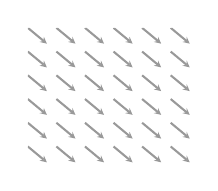
\begin{tikzpicture}[scale=.3]
 \begin{axis}[
major x tick style = transparent,
major y tick style = transparent,
x axis line style={transparent},
y axis line style={transparent},
xtick=\empty,
ytick=\empty,
zmin=0,zmax=1,
 domain=-.15:.15, view={0}{90}]
\addplot3[black!40,draw=black!40, quiver={u={1}, v={-1}, scale arrows=0.04, every arrow/.append style={line width=2.5pt*\pgfplotspointmetatransformed/1000}}, -stealth,samples=6, ] {0};
\end{axis}
 \end{tikzpicture}
\end{document}

\end{center}
Clearly \(Xu=0\) just when \(u\) satisfies our equation; but this happens just when \(u\) is 
constant along the flow lines of \(X\).
The flow lines of \(X\) are the diagonal lines, i.e. \(t+x\) constant, so
the solutions of our partial differential equation are \(u(t,x)=U(t+x)\) for any function \(U\).
Solutions of partial differential equations can involve arbitrary functions, as in this example.
Each solution \(u(t,x)\) is determined by its value at ``time'' \(t=0\).
If we pick our initial data function \(U\) not smooth at a point, then \(u(t,x)\) is not smooth along the flow line of that point.
So solutions can be worse than the initial data from which we construct them.

\begin{problem}{cauchy:vector.field}
Suppose that \(X\) is an analytic vector field on a manifold \(M\) and that \(H \subset M\) is an embedded analytic hypersurface and \(X\) is not tangent to \(H\) at any point of \(H\).
Pick analytic functions \(v \colon H \to \R\) and \(f \colon M \times \R \to \R\).
Prove that there is an analytic function \(u \colon \op{M} \to \R\) so that \(u(m,0)=v(m)\) for \(m \in H\) and \(Xu(m)=f(m,u(m))\) wherever \(u\) is defined.
Prove that any two such functions \(u=u_1\) and \(u=u_2\) agree near \(H\).
\end{problem}

\begin{example}
Take the differential equation \(u_t=u^2+t\).
Differentiate both sides:
\begin{align*}
u_{tt}
=&
2u \, u_t + 1, \\
=&
2u \, \pr{u^2+t} + 1.
\end{align*}
Our differential equation allows us to replace differentiation in \(t\) with some expression without any derivatives.
\end{example}
\begin{example}
The differential equation \(u_t = u^2 u_{xx} + \sin(u)\) allows us, using the chain rule, to replace any number of \(t\) derivatives by complicated expressions in \(x\) derivatives.
We can calculate any Taylor coefficient in any power of \(t\) as a function of finitely many Taylor coefficients involving only powers of \(x\), i.e. Taylor coefficients of \(u(x,0)\).
Danger: after we compute all of the Taylor coefficients, we have \emph{no guarantee} that they sum up to a convergent Taylor series.
\end{example}

A \emph{formal solution}\define{formal!solution}\define{solution!formal} of an analytic differential equation is a formal Taylor series so that expanding out the compositions term by term, all terms in the equation turn to zeroes.
As above, for any formal Tayor series \(u(0,x)\), there is an associated formal Taylor series solution \(u(t,x)\) of each partial differential equation \(u_t = f\of{t,x,u,u_x,u_{xx},\dots,u_{x\dots x}}\) for any smooth function or formal Taylor series \(f\).

\begin{example}
The heat equation \(u_t=u_{xx}\) has a unique formal Taylor series solution with intial condition
\[
 \left.u\right|_{t=0}= \frac{1}{1+x^2},
\]
given by
\[
 u(t,x)=\sum_{j,k=0}^{\infty} (-1)^{j+k}(2(j+k))! \frac{t^j}{j!} \frac{x^{2k}}{(2k)!}
\]
which doesn't converge anywhere except at \(t=0\).
\end{example}


\section{The method of majorants}
\begin{theorem}[Cauchy--Kovalevskaya]%
\label{theorem:Cauchy.Kovalevksaya}%
\define{theorem!Cauchy--Kovalevskaya}%
\define{Cauchy--Kovalevskaya theorem}%
An analytic system of partial differential equations of the form \(u_t=f\of{t,x,u,u_x}\), defined in an open set of \(t \in \R, x \in \R[n], u \in \R[p]\), with any analytic initial conditions \(u=U(x)\) at \(t=t_0\), has an analytic solution near \(t=t_0\).
Any two solutions agree near \(t=t_0\).
\end{theorem}
\begin{proof}
Instead of looking at Taylor series of solutions, look at Taylor series of equations.
Start with a simpler problem: take a differential equation \(u_t=f(t,u)\) with initial condition \(u(0)=u_0\).
Go back to our expressions for Taylor coefficients:
\begin{align*}
 u_t(0) &= f\of{0,u_0}, \\
 u_{tt}(0) &=f_t\of{0,u_0}+f_u\of{0,u_0}u_t, \\
 &=f_t\of{0,u_0}+f_u\of{0,u_0}f\of{0,u_0}, \\
 u_{ttt}(0)&= \dots. 
\end{align*}
If \(u_0 \ge 0\) and all of the Taylor coefficients of \(f\) are \(\ge 0\) then inductively all of the Taylor coefficients of \(u\) are \(\ge 0\).
In other words, if \(u_0 \ge 0\) and \(f\) majorizes \(0\) then \(u\) majorizes \(0\).

By the same reasoning, if we have two differential equations \(u_t=f(t,u)\) and \(v_t=g(t,v)\) with initial conditions \(u(0) \ge v(0)\), and if \(f\) majorizes \(g\), then by the same induction, \(u\) majorizes \(v\).
In particular, if the Taylor series of \(u\) converges, then so does that of \(v\).
\begin{problem}{cauchy:check.series.2}
 Check that the function
 \[
  u(t)=1-\sqrt{1+2 \log(1-t)}
 \]
 satisfies the \emph{toy} equation
 \[
  u_t = \frac{1}{(1-t)(1-u)}
 \]
 with initial condition \(u=0\) at \(t=0\).
\end{problem}

Don't expand the unpleasant function \(u(t)\) but expand the toy equation
\begin{align*}
  u_t=&\frac{1}{(1-t)(1-u)},\\ 
  =&\pr{1+t+t^2+\dots}\pr{1+u+u^2+\dots}, \\
  =&\sum_{jk} t^ju^k:
\end{align*}
a geometric series.
Suitable rescaling of \(t\) and \(u\) produces any convergent geometric series we like.
By lemma~\vref{lemma:cauchy:convergent.Taylor}, any analytic function \(f(t,u)\) is majorized by a geometric series in \(t,u\).
So the equation \(u_t=f(t,u)\) is majorized by the toy equation, after some rescaling of variables.
So the solution \(u(t)\) to \(u_t=f(t,u)\) with \(u(0)=0\) is majorized by the toy solution, so has convergent Taylor series.

We will generalize this toy example several times, to get a larger class of examples of majorizing equations.
The function
\[
 u(t,x)=1-x-\sqrt{(1-x)^2-2t}
\]
satisfies
\[
 u_t=\frac{1+u_x}{1-x}
\]
with \(u=0\) at \(t=0\).
With suitable rescalings of \(x,t,u\), this equation majorizes any equation of the form \(u_t=f\of{x,u}+g\of{x,u}u_x\) for any analytic \(f, g\), with \(x,u \in \R\) in a suitable open set.
Therefore all such equations have local analytic solutions so that \(u=0\) when \(t=0\).

To allow more \(x\) variables: if \(u(t,s)\) is the function above
\[
 u(t,s)=1-s-\sqrt{(1-s)^2-2t} 
\]
and we let \(v(t,x)=u(t,s)\) where we let \(s=\sum_i x_i\) where \(x \in \R[n]\), then 
\[
 v_t = \frac{1+\frac{1}{n}\sum v_{x_i}}{1-\sum x_i}
\]
and \(v=0\) at \(t=0\).
Again, with a little rescaling, this equation majorizes any equation of the form \(u_t=f\of{x,u}+g\of{x,u}u_x\) for any analytic \(f, g\), and \(t,u \in \R\), \(x \in \R[n]\) in some open set.
Of course the same trick works even if we allow many \(u\) functions, i.e. \(u \in \R[p]\).

To allow the \(t\) variable to enter into the right hand side, we add a new equation \(v_t=1\) with initial condition \(v=0\) at \(t=0\), so we are just forcing \(v=t\) everywhere.
Then any system like \(u_t=f(t,x,u)+g(t,x,u)u_x\) with \(u=0\) when \(t=0\) is equivalent to 
\begin{align*}
 u_t=&f(v,x,u)+g(v,x,u)u_x, \\
 v_t=&1,
\end{align*}
with \(u=v=0\) when \(t=0\).
We have already seen that such systems have solutions near the origin, 

If we want to solve a system of the form \(u_t=f\of{t,x,u,u_x}\), invent a new variable \(v\) and solve instead
\begin{align*}
u_t &= f\of{t,x,u,v}, \\
v_t &= f_x\of{t,x,u,v} + f_u\of{t,x,u,v}v+f_v\of{t,x,u,v}v_x,
\end{align*}
with \(u=v=0\) when \(t=0\), to force \(v=u_x\).

Suppose that we want to solve a system \(u_t=f(t,x,u,u_x)\) with \(u=U(x)\) at \(t=0\) instead of \(u=0\) at \(t=0\).
Replace the system by the system \(v_t=f(t,x,v+U,v_x+U_x)\) with \(v=0\) at \(t=0\) and then let \(u(t,x)=v(t,x)+U(x)\).
\end{proof}
\begin{example}
Given a solution \(u\) to the wave equation \(u_{tt} = u_{xx}\) with initial conditions \(u=U\) and \(u_t=W\) at \(t=0\), let
\[
   v(t,x)=\int W(x) \, dx + \int_0^t u_x(s,x) \, ds
\]
so that \(v_t=u_x\).
Differentiate under the integral sign and apply the fundamental theorem of calculus to find that \(v_x=u_t\).
Therefore \(u,v\) satisfy
\begin{align*}
  u_t &= v_x, \\
  v_t &= u_x
\end{align*}
with initial conditions \(u=U\) and \(v=W\) at \(t=0\).
Conversely, any solution to this system of equations recovers our solution \(u\) to the wave equation.
An analytic solution of the wave equation is uniquely determined by the initial height and velocity of the waves.
\end{example}
To solve a second order system \[u_{tt}=f\of{t,x,u,u_x,u_t,u_{xx},u_{xt}},\] with initial conditions \(u=U(x)\) and \(u_x=W(x)\) at \(t=0\), let \(p=u_x\) and \(q=u_t\).
Then
\begin{align*}
u_t &= q, \\
p_t &= q_x, \\
q_t &= f\of{t,x,u,p,q,p_x,q_x},
\end{align*}
with initial conditions \(u=U(x)\), \(p=U'(x)\), \(q=W(x)\) at \(t=0\).
Any solution or formal solution of this system arises from a solution or formal solution to the original system and vice versa.
This same trick reduces any system of any order to a first order system in more variables.
\begin{example}
Is there a vector field \(u\) so that \(\nabla \times u = f\) for a given vector field \(f\) in \(\E[3]\)?
Write \(u=\pr{u^1,u^2,u^3}\) and \(f=\pr{f^1,f^2,f^3}\) and let
\[
u^1_{x_2} \defeq \pderiv{u^1}{x_2}, \text{etc}.
\]
Our equation \(\nabla \times u = f\) expands out to
\begin{align*}
u^3_{x_2}-u^2_{x_3} &= f^1, \\
u^1_{x_3}-u^3_{x_1} &= f^2, \\
u^2_{x_1}-u^1_{x_2} &= f^3:
\end{align*}
\(3\) first order equations for \(3\) unknowns.
By analogy with the Cauchy--Kovalevskaya theorem, we expect to find a unique solution with initial values of \(u^1, u^2, u^3\) given on some surface in \(\E[3]_{x_1, x_2, x_3}\).
This expectation is \emph{not} correct.
Taking \(\nabla \cdot\) on both sides of our equations reveals \(0=\nabla \cdot f\).
If \(0\ne \nabla \cdot f\) then there is no solution \(u\).
If \(0=\nabla \cdot f\) then the solutions are \(u=u_0 + \nabla \phi\) 
for any one fixed solution \(u_0\) and for any twice continuously differentiable function \(\phi\).
So the local solutions depend on one function \(\phi\) of \(3\) variables, not on initial data from a surface in \(\E[3]\).

We might spot trouble on the horizon when we notice that we can't solve our equations for the derivatives with respect to \(x_1\), since there are only two of them, and similarly for \(x_2\) and for \(x_3\).
Nonetheless, we can easily make more complicated examples of systems of partial differential equations to which the Cauchy--Kovalevskaya theorem does not apply, with complicated ``compatibility conditions'' needed to ensure existence of a solution.
\end{example}

\begin{example}\label{page:nabla.u.f.u}
Is there a vector field \(u\) so that \(\nabla \times u = f - u\) for a given vector field \(f\) in \(\E[3]\)?
Our equation \(\nabla \times u = f - u\) expands out to
\begin{align*}
u^3_{x_2}-u^2_{x_3} &= f^1 - u^1, \\
u^1_{x_3}-u^3_{x_1} &= f^2 - u^2, \\
u^2_{x_1}-u^1_{x_2} &= f^3 - u^3:
\end{align*}
\(3\) first order equations for \(3\) unknowns.
Again we might expect to find a unique solution with initial values of \(u^1, u^2, u^3\) given on some surface in \(\E[3]_{x_1, x_2, x_3}\).
Again this intuition is \emph{not} correct.
Taking \(\nabla \cdot\) on both sides of our equations reveals \(0=\nabla \cdot f - \nabla \cdot u\), i.e.
\[
u^1_{x_1} + u^2_{x_2} + u^3_{x_3}
=
f^1_{x_1} + f^2_{x_2} + f^3_{x_3},
\]
a fourth first-order equation which is linearly independent of the other three.

Split the four equations as:
\begin{align*}
u^3_{x_2}-u^2_{x_3} &= f^1 - u^1, \\
\intertext{and}
u^1_{x_3}-u^3_{x_1} &= f^2 - u^2, \\
u^2_{x_1}-u^1_{x_2} &= f^3 - u^3, \\
u^1_{x_1} + u^2_{x_2} + u^3_{x_3} &=
f^1_{x_1} + f^2_{x_2} + f^3_{x_3}.
\end{align*}
Solve the first of these equations:
\[
u^3_{x_2}-u^2_{x_3} = f^1 - u^1,
\]
but just along the surface \(x_1=0\), using the Cauchy--Kovalevskaya theorem in the variables \(x_2, x_3\), starting with any choice of functions \(u^1, u^2\) on the surface \(x_1=0\) and any function \(u^3\) on the curve \(x_1=x_2=0\).
Apply the Cauchy--Kovalevskaya theorem to the last \(3\) equations:
\begin{align*}
u^1_{x_3}-u^3_{x_1} &= f^2 - u^2, \\
u^2_{x_1}-u^1_{x_2} &= f^3 - u^3, \\
u^1_{x_1} + u^2_{x_2} + u^3_{x_3} &=
f^1_{x_1} + f^2_{x_2} + f^3_{x_3}.
\end{align*}
in all \(3\) variables \(x_1, x_2, x_3\), by treating \(x_1\) as the variable we differentiate in:
\[
\begin{pmatrix}
u^1 \\
u^2 \\
u^3
\end{pmatrix}
_{x_1}
=
\begin{pmatrix}
- u^2_{x_2} - u^3_{x_3} + \nabla \cdot f \\
u^1_{x_2} + f^3 - u^3, \\
u^1_{x_3} - f^2 + u^2
\end{pmatrix}.
\]
The tricky question is whether the resulting functions actually solve the original problem.
In fact, they do: we have solved the first equation
\[
u^3_{x_2}-u^2_{x_3} = f^1 - u^1,
\]
at \(x_1=0\).
But if we differentiate that expression in \(x_1\), check that
\[
\pr{u^3_{x_2}-u^2_{x_3} - f^1 + u^1}_{x_1}
=
0
\]
modulo the \(3\) other equations, so vanishes by construction.
The general solution to \(\nabla \times u = f - u\) is given by picking one arbitrary function of one variable, and \(2\) arbitrary functions of two variables, again not what we would guess from familiarity with the Cauchy--Kovalevskaya theorem.

Again, we might spot trouble on the horizon when we notice that we can't solve our equations for the derivatives with respect to \(x_1\), since there are only two of them, and similarly for \(x_2\) and for \(x_3\).
\end{example}

\section{Smooth counterexamples}
For functions which are not analytic, there are numerous theorems to prove the existence of solutions, under a wide variety of hypotheses, but there are some surprising counterexamples:
\begin{enumerate}
\item
The Cauchy--Riemann equations admit only analytic solutions: no solution has smooth nonanalytic initial data.
\item
Some linear determined equations \(Lu=f\) with analytic \(L\) have no solutions for any smooth \(f\) unless \(f\) is analytic \cite{Lewy:1957}.
\end{enumerate}
